\section{Workload Characterization}
\label{sec:motivation}

\subsection{Analysis of Post-Transformer LLMs}
\label{subsec:state_update_characterization}
%
\niparagraph{Common operational structure.}
%
As discussed in Section~\ref{subsec:ssm_based_llms}, many
post-transformer models exhibit a shared structured pattern that is
increasingly evident in recent algorithms.
%
We find that we can unify this shared algorithmic commonality across
post-transformer models into a single, generalized operation, termed
\textbf{state update}.
%
For clarity, we refer to post-transformer models employing this state
update as \textbf{\underline{S}}tate
\textbf{\underline{U}}pdate-based \textbf{\underline{LLMs}}, or
\textbf{SU-LLMs} for short.
%
Equation~\ref{eq:state_update} represents the state update operation
for a single head.
%
\begin{equation}
  \label{eq:state_update}
  \begin{aligned}
    &S_t = d_t \odot S_{t-1} + k_t v_t^T \\
    &y_t = S_t^T q_t
  \end{aligned}
\end{equation}
%
Here, $d_t$, $q_t$, and $k_t$ are vectors with $dim_{head}$
dimension, while $v_t$ is a vector with $dim_{state}$ dimension.
%
The state is represented as a matrix of ($dim_{head} \times
dim_{state}$) dimensions.
%
First, the $d_t$ vector is broadcast to match the dimensions of the
state matrix, after which an element-wise multiplication is performed
to decay the state.
%
This decayed state is then updated by adding the outer product of
$k_t$ and $v_t$.
%
The updated state is then multiplied by $q_t$ using GEMV to produce
the output $y_t$.
%

\begin{figure*}[t]
  \centering
  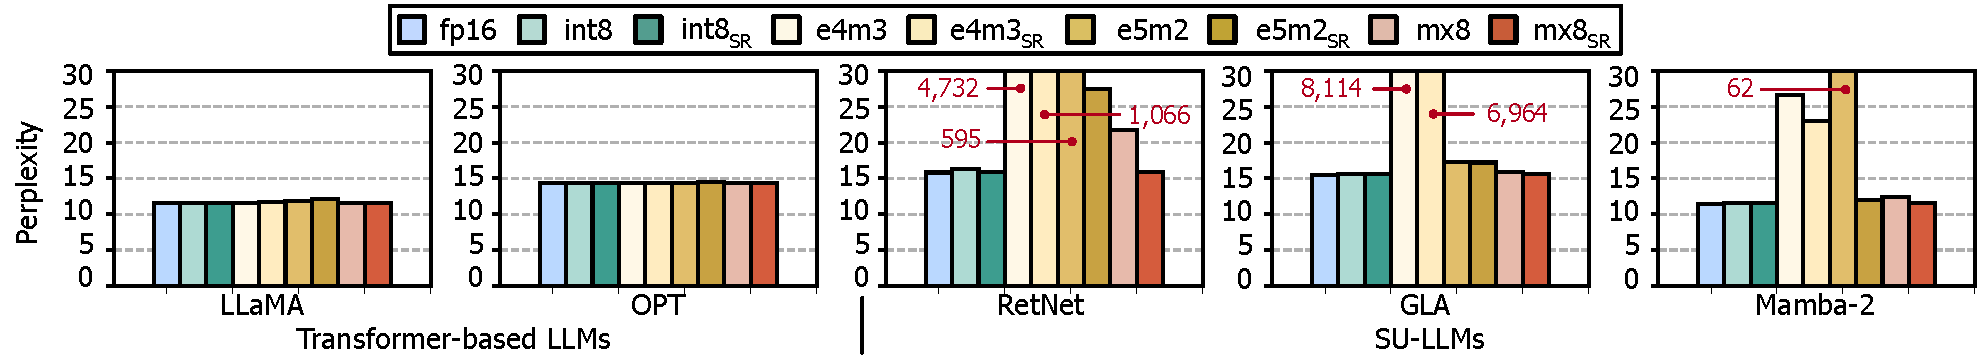
\includegraphics[width=\linewidth]{fig/characterization_quant.pdf}
  \caption{Perplexity of SU-LLMs and transformer-based LLMs using the
    WikTtext-2~\cite{merity2016pointer} dataset when quantized their
  respective representations to 8-bit formats.}
  \label{fig:characterization_quant}
\end{figure*}
%

%
\niparagraph{Performance Analysis.}
%
Figure~\ref{fig:motivation_breakdown} illustrates the latency
breakdown of operations during generation phase across 2.7B parameter
SU-LLMs--such as RetNet, GLA, HGRN2, Mamba-2~\cite{retnet,
gated_linear_attention, hgrn2, mamba2}--along with
Zamba2~\cite{zamba2}, a 7B parameter hybrid transformer-Mamba-2 model
using A100 GPU.
%
Unless otherwise specified, we use models with the same parameter
count throughout this paper.
%
The results show that state updates dominate latency, despite having
fixed memory and compute footprints.
%
In RetNet, as the batch size increases from 32 to 128, the time spent
on state updates rises from 41.9\% to 73.8\%, resulting in a
significant bottleneck.
%
This is because state updates are memory-bound and lack parameter
reuse across user requests.
%
They read and write the state matrix, while each operation--such as
decay, outer product, update, and GEMV--requires FLOPs proportional
to the size of the state matrix, resulting in a low operational intensity.
%
Furthermore, each request must independently read, update, and write
its own state.
%
Consequently, their latency grows linearly with batch size, rendering
state updates a performance bottleneck at large batch sizes.
%

%
Another noteworthy observation is that in a hybrid model such as
Zamba2, although the number of Mamba-2 layers greatly exceeds that of
attention layers (e.g. 6$\times$), attention still represents a
substantial fraction of the overall latency--reaching 65.5\% at a
batch size of 128.
%
This is because, unlike state update operations that exhibit constant
latency regardless of sequence length, attention operations scale in
latency proportionally to sequence length, making them a dominant
bottleneck in long-sequence scenarios.
%
Hence, to effectively accelerate hybrid models, it is critical to
optimize not only state update operations but also attention operations.
%

\subsection{Quantization Analysis for SU-LLMs}
\label{subsec:challenges_quantization}
%
As discussed in Section~\ref{subsec:state_update_characterization},
state update operations are memory-bound, leading to significant
memory bandwidth pressure.
%
Quantizing the state may offer a promising solution to mitigate this
issue by reducing data precision and thus memory bandwidth needs.
%
Although significant research has been dedicated to quantizing the KV
cache in transformer-based LLMs~\cite{xiao2023smoothquant,
hooper2024kvquant, atom}, the quantization of the state in SU-LLMs
has received little attention.
%

%
\niparagraph{Low precision formats.}
%
To address this gap, we explore various low-precision formats for
quantizing the state: (1) integer, (2) floating point, and (3) block
floating point formats.
%
For the integer format, we use an 8-bit integer with a scaling factor
across every 32 elements.
%
For the floating point format, we consider 8-bit variants:
\texttt{e4m3} (4 exponent bits and 3 mantissa bits) and \texttt{e5m2}
(5 exponent bits and 2 mantissa bits).
%
For the block floating point format, we employ
\texttt{MX}~\cite{rouhani2023shared}.
%
Specifically, we employ a variant of \texttt{MX}, called
\texttt{MX8}, where groups of 16 values share a common 8-bit
exponent, and pairs of values within each group share a 1-bit
microexponent to match the bit-width.
%
We also investigate the impact of rounding methods, particularly
stochastic rounding, which rounds numbers probabilistically based on
their distance from representable values.
%

%
\niparagraph{Implication of quantization for SU-LLMs.}
%
Figure~\ref{fig:characterization_quant} shows the perplexity of
various 2.7B parameter models when their respective
representations--state for SU-LLMs and KV cache for transformers--are
quantized using the Wikitext-2~\cite{merity2016pointer} dataset.
%
Our results reveal distinct quantization behaviors between these two
model types.
%

%
Transformer-based LLMs exhibit negligible perplexity increases across
all formats, while SU-LLMs exhibit a severe increase in perplexity
with floating point formats (e.g. 8,114 for GLA with \texttt{e4m3}).
%
This discrepancy arises from the SU-LLMs' continuous state ``update'' mechanism.
%
This makes them vulnerable to loss of small values during
accumulation due to limited mantissa precision, which is called
swamping effect~\cite{swamping, wang2018training}.
%
The 7-bit (\texttt{int8}) and 6-bit (\texttt{MX8}) mantissas provide
enough precision to mitigate swamping, whereas the 3-bit and 2-bit
mantissas in \texttt{e4m3} and \texttt{e5m2} render these formats
highly susceptible.
%
This finding aligns with conventional practices in training deep
learning models, wherein weights are stored at higher precisions to
reduce numerical errors~\cite{micikevicius2018mixed}.
%
Another notable observation is that stochastic rounding has a
substantial positive impact on SU-LLMs, in contrast to transformer-based LLMs.
%
For example, the perplexity of Mamba-2 in the \texttt{e5m2} format
drops dramatically from 62 to 11.9 when stochastic rounding is applied.
%
In SU-LLMs, stochastic rounding probabilistically preserves smaller
magnitude values that would otherwise be lost due to swamping,
thereby maintaining more information during state update scenario.
%

%
According to the results, employing stochastic rounding on
\texttt{int8} appears optimal for SU-LLMs.
%
However, this strategy might require re-evaluation in
area-constrained environments, such as PIM architectures.
%
We will discuss this in further detail in Section~\ref{subsec:area_accuracy}.
%

\begin{figure}[t]
  \centering
  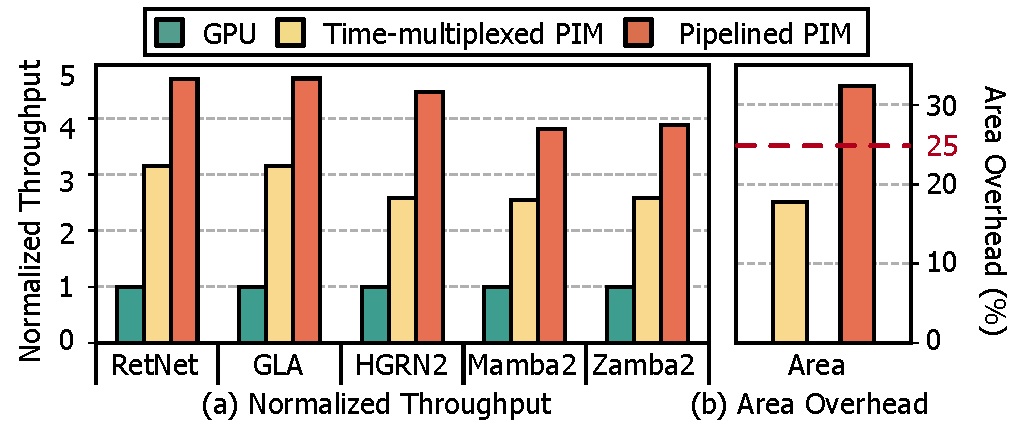
\includegraphics[width=\linewidth]{fig/challenges_pim.pdf}
  \caption{(a) Normalized throughput for state updates of various
  SU-LLMs. (b) Area overhead for two PIM designs.}
  \label{fig:challenges_pim}
\end{figure}
%
\begin{figure}[t]
  \centering
  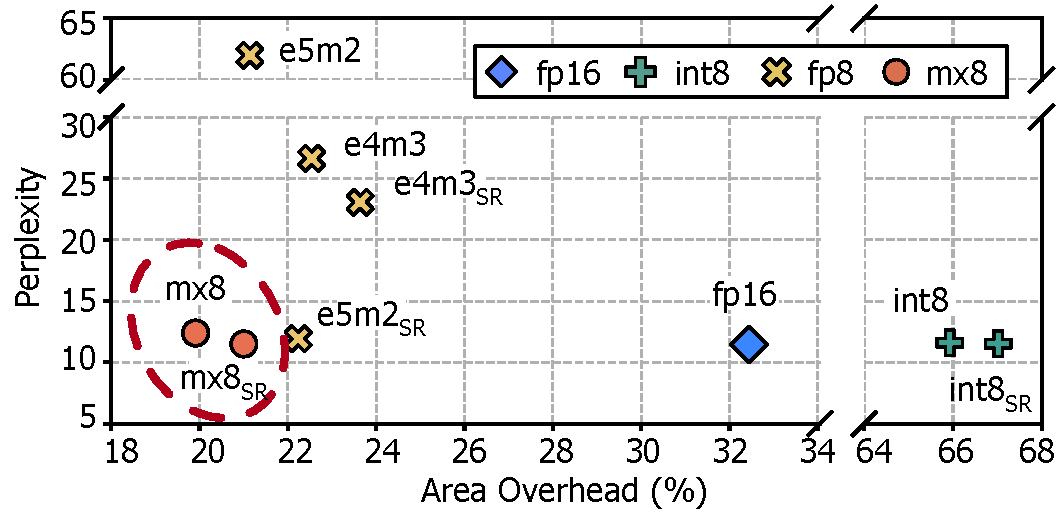
\includegraphics[width=\linewidth]{fig/quantization_pareto.pdf}
  \caption{Accuracy-area tradeoff between different low-precision
    formats on Mamba-2 model with WikiText-2. All compute units take
  256-bit-group operands as input.}
  \label{fig:quantization_pareto}
\end{figure}
%
\begin{figure*}[t]
  \centering
  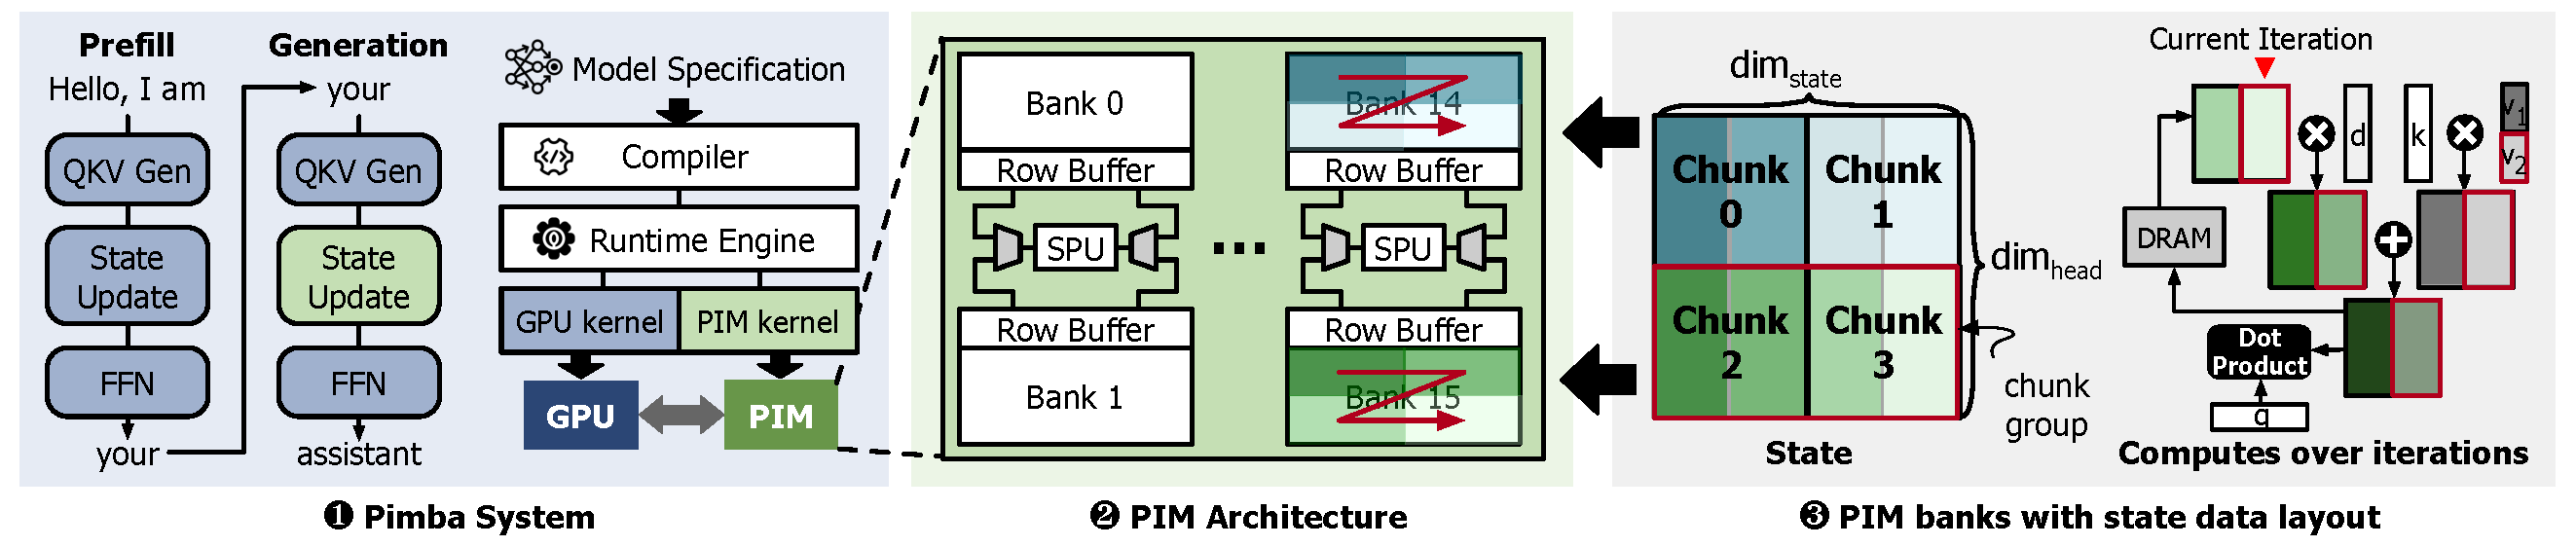
\includegraphics[width=\linewidth]{fig/overview_system.pdf}
  \caption{Overview of the proposed \sysname{} system.}
  \vspace{-1ex}
  \label{fig:overview_system}
\end{figure*}
